\documentclass[a4paper,12pt]{report}
\usepackage[T2A]{fontenc}
\usepackage[utf8]{inputenc}
\usepackage[english,russian]{babel}
\usepackage{graphicx}
\usepackage{wrapfig}
\usepackage{mathtext} 				% русские буквы в фомулах
\usepackage{amsmath,amsfonts,amssymb,amsthm,mathtools} % AMS
\usepackage{icomma} % "Умная" запятая: $0,2$ --- число, $0, 2$ --- перечисление
\usepackage{capt-of}
\usepackage{appendix}
\usepackage{multirow}
\usepackage{hyperref}
\usepackage{floatrow}
\usepackage[left=2cm,right=2cm,
    top=2cm,bottom=2cm,bindingoffset=0cm]{geometry}
\usepackage{multicol} % Несколько колонок
\usepackage{gensymb}
\title{Отчёт по лабораторной работе №11

Исследование работы сдвигового регистра на цилиндрических магнитных доменах}
\author{Плюскова Н.А. Б04-004 }
\date{\today}

\begin{document}

\maketitle

\section*{1. Аннотация}
В данной работе была найдена область работоспособности элемента запоминающего устройства и изображен соответствующий график.

\section*{2. Теоретические данные}
Ферромагнитный кристалл в отсутствие внешнего поля разбивается на области спонтанной намагниченности - домены, в пределах которых намагниченность постоянна. В следствие анизотропии кристалла появляется легкая ось намагничивания (ОЛН).

$\textbf{Как можно представить происхождение магнитной анизотропии?}$

Намагниченность создается суммированием элементарных магнитных моментов атомов (или ионов) кристалла. Электроны, определяющие намагниченность, характеризуются помимо спиновых и орбитальных моментами, последние связаны с кристаллографическими направлениями. Благодаря спин-орбитальному взаимодействию, спиновые магнитные моменты удерживаются вдоль определенных кристаллографических осей. В этом основная причина магнитокристаллической анизотропии. Анизотропии типа "легкая ось" присуща определенная энергия $E_a = -Kcos^2\varphi$, где $\varphi$ - угол между намагниченностью и ОЛН, а $K>0$, так называемая константа одноосной анизотропии. Понятно, что K - величина энергетического барьера между двумя противоположными состояниями в равной энергией вдоль ОЛН.

$\textbf{Условия статической устойчивости изолированных цилиндрических магнитных}$
$\textbf{доменов (ЦМД)}$

Представим себе, что в тонкой монокристаллической пластине или пленке, намагниченной до насыщения вдоль ОЛН, каким-то образом создана область с противоположным направлением намагниченности. Логично предположить, что эта область будет иметь цилиндрическую форму ЦМД.

Для определения условий равновесного существования указанной области и интервала устойчивости по магнитному полю нужно провести анализ системы домен в пластине на устойчивость. Для этого диаметр домена $d$ представляют в виде ряда Фурье.
Уравнение равновесия круглого ЦМД, определяемое из условия обращения в нуль вариации полной энергии, имеет вид:
\begin{equation}
    F_{w} + \frac{d}{h}\cdot\frac{H}{M} - F(\frac{d}{h}) = 0,
\end{equation}
где $F_{w} = \frac{\partial E}{\partial d}(\pi \mu_{0} M^2h^2)^{-1}$ - нормированная обобщенная сила поверхностного натяжения на границу раздела двух магнитных фаз, $F(\frac{d}{h})$ - обобщенная нормарованная магнитостатическая сила (силовая функция).

Таким образом уравнение (1) есть уравнение устойчивости ЦМД с линейной структурой доменной стенки. Введя $l = \sigma_{0}\mu_{0}^{-1}M^2$ (характеристическую длину материала), уравнение (1) можно переписать:

\begin{equation}
    \frac{l}{h} + \frac{d}{h}(\frac{H}{M}) = F(\frac{d}{h})
\end{equation}

Равновесный диаметр и интервал полей устойчивого состояния изолированного ЦМД можно определить, решив (2) графически (см. рис.1) Диаметры устойчивых ЦМД устойчивых ЦМД заключены внутри отрезка, который образуется при пересечении горизонтальной прямой $y = \frac{l}{h} + \frac{d}{h}(\frac{H}{M})$ с кривой $F(\frac{d}{h})$. Левая точка пересечения соответствует неустойчивому решению. Нижняя граница интервала устойчивости ЦМД по полю подмагничивания определяется $\textit{эллиптической неустойчивостью}$, верхняя - соответствует $\textit{коллапсу ЦМД}$

\begin{figure}[H]
\centering
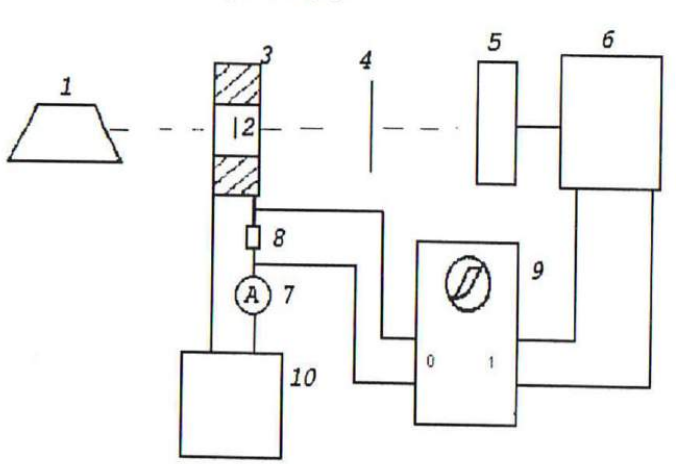
\includegraphics[width=0.7\linewidth]{pic3.png}
\caption{Графики функций стабильность $S_{0}$ и $S_{2}$ и силовой функции $F$}
\end{figure}

\textbf{Принципы управления ЦМД}

Чтобы обеспечить перенос двоичной информации, закодированной в виде ЦМД, нужно создавать условия, обеспечивающие его перемещение, что возможно с помощью локальных магнитных полей, эффективно действующих на границу ЦМД. Для создания таких полей в ЦМД-схемах предназначены так называемые управляющие элементы, примером которых являются намагничиваемые внешним однородным полем-Н управляющим - участки ферромагнитной пленки-аппликации.

\begin{figure}[H]
\centering
\includegraphics[width=0.7\linewidth]{application.jpg}
\caption{Перемещение ЦМД вдоль пермаллоевой аппликации}
\end{figure}

Рассмотрим, как распределяются поля, действующие со стороны намагниченной аппликации на ЦМД. Если магнитное поле намагниченного управляющего элемента-аппликации имеет $z$-компоненту, ориентированную вдоль поля смещения Н$_{\text{см}}$ (значения Н$_{\text{см}}$ обеспечивают устойчивые состояния ЦМД) и противоположную ему по знаку, в ЦМД-материале возникает область пониженных значений Н$_{\text{см}}$, называемая магнитостатической ловушкой (МСЛ). Если совпадает по знаку с Н$_{\text{см}}$, говорят о магнитостатическом барьере (МСБ). 

%На рис. 5а показана качественная картина распределения напряженности поля рассеяния намагниченной прямоугольной аппликации, в каждой точке которого можно выделить вертикальную Н$_{z}$ а горизонтальную Н$_{x}$ компоненты. Аппликация размещается над поверхностью ЦМД-пленки на расстоянии, определяемые толщиной защищающего ЦМД-пленку диэлектрика. При попадании ЦМД в МСЛ уменьшается его полная энергия, т.е. ЦМД оказывается в потенциальной яме, его радиус при этом несколько увеличивается.

Аппликации канала изготавливаются из изотропного магнитомягкого пермаллоя толщиной около 0,5 мкм с малым значением коэрцитивной силы. Ширина пермаллоевых полосок схем управления движением составляет примерно половину диаметра ЦМД, период структуры от 3 до 4 d. Самым узким местом в изготовлении аппликаций является зазор между соседними элементами, который обычно составляет около 2/3 ширины пермаллоевой полоски.

\textbf{Область работоспособности}

Под областью работоспособности (ОРС) элемента запоминающего устройства на ЦМД или областью устойчивой работы	понимается множество пар значений полей смещения Н$_{\text{см}}$ и вращения Н$_{\text{вр}}$, при которых элемент функционирует без искажения информации. Левая граница определяет то минимальное поле вращения Н$_{\text{вр}}$, при котором ЦМД способны перемещаться посредством пермаллоевых аппликаций. Правая граница определяется значениями поля вращения, при которых происходит самопроизвольное зарождение ЦМД под пермаллоевыми аппликациями. Верхняя граница зависит от значений поля смещения, при которых в данном элементе наступает коллапс ЦМД. Нижняя граница - граница эллиптической неустойчивости - соответствует значениям поля смещения, при которых цилиндрический домен неуправляемо растягивается в полосовой домен.

\begin{figure}[H]
\centering
\includegraphics[width=0.7\linewidth]{work.jpg}
\caption{Примерная область работоспособности линейного участка элемента продвижения}
\label{theory}
\end{figure}

\section*{3. Результаты эксперимента и обработка данных}
После настойки микроскопа и его юстировки, а также настройки экспериментальной установки (в нашей лабе уже было сделано). Определим граничные точки по полю смещения ОРС элемента продвижения (каждые измерения проводились трижды, после чего были усреднены):

\begin{table}[]
\begin{tabular}{|l|l|l|}
\hline
H$_{\text{вр}}$, э & H$_{\text{см}}$ верхняя точка, э & Н$_{\text{см}}$ нижняя точка, э \\ \hline
49     & 146,5                & 106,5               \\ \hline
44     & 139                  & 94,5                \\ \hline
39     & 134,5                & 88,5                \\ \hline
34     & 131                  & 91,5                \\ \hline
29     & 124                  & 94,5                \\ \hline
24     & 128,5                & 87                  \\ \hline
19     & 127,5                & 88,5                \\ \hline
14     & 118,5                & 88,5                \\ \hline
9      & 112,5                & 89,5                \\ \hline
4      & 102                  & 92                  \\ \hline
\end{tabular}
\end{table}

Построим соответствующий график и проведем аппроксимацию:

\begin{figure}[H]
\centering
\includegraphics[width=0.7\linewidth]{no-appr.jpg}
\caption{Зависимость H$_{\text{см}}$ от H$_{\text{вр}}$}
\label{no-appr}
\end{figure}
\begin{figure}[H]
\centering
\includegraphics[width=0.7\linewidth]{app.jpg}
\caption{Аппроксимация зависимости H$_{\text{см}}$ от H$_{\text{вр}}$}
\label{appr}
\end{figure}

\section*{4. Вывод}
В ходе работы нам удалось рассмотреть процесс движения ЦМД в сдвиговом регистре, найти его область работоспособности; полученные результаты приведены в виде графика на рисунке \ref{no-appr}, их вид соответствует теоретической модели, что продемонстрировано на рисунке \ref{appr}.

%Для Влада:
%Во время выполнения работы мы смогли изучить процесс движения ЦМД в сдвиговом регистре,а также найти его область работоспособности. Экспериментальные данные представлены на рисунках \ref{no-appr} и \ref{appr}, вид полученной зависимости совпадает с теоретической.

\end{document}
